%%%%%%%%%%%%%%%%%%%%%%%%%%%%%%%%%%%%

\section{4.5. Inferência para outras estimativas}

%%%%%%%%%%%%%%%%%%%%%%%%%%%%%%%%%%%%

\begin{frame}
\frametitle{Inferência para outras estimativas}

\begin{itemize}
\justifying
\item A média amostral não é a única estimativa pontual para a qual a distribuição amostral é quase normal. Por exemplo, a distribuição amostral das proporções da amostra também é quase normal quando $ n $ é suficientemente grande.
\justifying
\item Um pressuposto importante sobre as estimativas pontuais é que elas são \hl {imparciais}, ou seja, a distribuição amostral da estimativa é centrada no parâmetro populacional verdadeiro que se está estimando.

\begin{itemize}
\justifying
\item Ou seja, uma estimativa imparcial não sobrestima ou subestima o parâmetro. Em vez disso, ele tende a fornecer uma estimativa "boa".
\justifying
\item A média da amostra é um exemplo de uma estimativa pontual imparcial, assim como cada um dos exemplos que introduzimos nesta seção.
\end{itemize}
\end{itemize}
\end{frame}
%%%%%%%%%%%%%%%%%%%%%%%%%%%%%%%%%%%%

\begin{frame}
\frametitle{Inferência para outras estimativas}

\begin{itemize}
\justifying
\item Algumas estimativas pontuais seguem distribuições diferentes da distribuição normal, e alguns cenários requerem técnicas estatísticas que ainda não foram abordadas - discutiremos estas no final desta seção.

\end{itemize}

\end{frame}

%%%%%%%%%%%%%%%%%%%%%%%%%%%%%%%%%%%%

\subsection{Intervalos de confiança para estimativas pontuais quase normais}

%%%%%%%%%%%%%%%%%%%%%%%%%%%%%%%%%%%%

\begin{frame}
\frametitle{Intervalos de confiança para estimativas pontuais quase normais}
\justifying
Um intervalo de confiança baseado em uma estimativa pontual imparcial e quase normal é

\[ estimativa~pontual~ z^\star~ SE  \]
\justifying
onde $z^\star$ é selecionado para corresponder ao nível de confiança e SE representa o erro padrão.

$\:$ \\
\justifying
Lembre-se que o valor $z^\star~ SE$ é chamado de \hl{margem de erro}.

\end{frame}

%%%%%%%%%%%%%%%%%%%%%%%%%%%%%%%%%%%

\begin{frame}
\frametitle{Prática}

\justifying
\pq{Um dos primeiros exemplos de assimetria comportamental é uma preferência em humanos por virar a cabeça para a direita, e não para a esquerda, durante as últimas semanas de gestação e nos primeiros 6 meses após o nascimento. Acredita-se que isso influencie o desenvolvimento subsequente das preferências perceptivas e motoras. Um estudo de 124 casais descobriu que 64,5\% viravam a cabeça para a direita quando se beijavam. O erro padrão associado a essa estimativa é de aproximadamente 4\%. Qual das opções abaixo é \emph{falsa}?}

\end{frame}
%%%%%%%%%%%%%%%%%%%%%%%%%%%%%%%%%%%

\begin{frame}

\frametitle{Prática}

\begin{enumerate}[(a)]
\justifying
\solnMult{O intervalo de confiança de 95\% para a porcentagem de casais que durante o beijo viram suas cabeças para a direita é aproximadamente $64.5\% \pm 4\%$.}
\justifying
\item Um tamanho de amostra maior produziria um erro padrão menor.
\justifying
\item A margem de erro para um intervalo de confiança de 95\% para a porcentagem de casais que durante o beijo viram a cabeça para a direita é de aproximadamente 8\%.
\justifying
\item O intervalo de confiança de 99,7\% para a porcentagem de casais que durante o beijo viram a cabeça para a direita é aproximadamente $64.5\% \pm 12\%$.
\end{enumerate}


\vfill
\justifying
\ct{G\"{u}nt\"{u}rk\"{u}n, O. (2003) Adult persistence of head-turning asymmetry. \textit{Nature}. Vol 421.}

\end{frame}

%%%%%%%%%%%%%%%%%%%%%%%%%%%%%%%%%%%%

\subsection{Teste de hipóteses para estimativas pontuais quase normais}

%%%%%%%%%%%%%%%%%%%%%%%%%%%%%%%%%%%

\begin{frame}
\frametitle{Teste de hipóteses para estimativas pontuais quase normais}
\justifying
\dq{A terceira Pesquisa Nacional de Exame de Saúde e Nutrição coletou dados do percentual de gordura corporal (BF \%) e gênero de 13.601 indivíduos com idades entre 20 e 80 anos. A média de BF\% para os 6.580 homens da amostra foi de 23,9 e esse valor foi de 35,0 para as 7.021 mulheres. O erro padrão para a diferença entre a média do BF\%s de homens e mulheres foi de 0,114. Esses dados fornecem evidências convincentes de que homens e mulheres têm médias diferentes de BF\%s. Você pode assumir que a distribuição da estimativa pontual é quase normal.}

\end{frame}
%%%%%%%%%%%%%%%%%%%%%%%%%%%%%%%%%%%
\begin{frame}
\frametitle{Teste de hipóteses para estimativas pontuais quase normais}

\begin{enumerate}
\justifying
\item[1.] Definir hipóteses
\justifying
\item[2.] Calcular estimativa pontual
\justifying
\item[3.] Verificar condições
\justifying
\item[4.] Desenhar distribuição amostral, sombrear o p-valor
\justifying
\item[5.] Calcular estatísticas de teste e o p-valor, tomar uma decisão
\end{enumerate}

\end{frame}

%%%%%%%%%%%%%%%%%%%%%%%%%%%%%%%%%%%

\begin{frame}
\frametitle{Teste de hipóteses para estimativas pontuais quase normais}

\begin{enumerate}
\justifying
\item[1.] A hipótese nula é que homens e mulheres têm a mesma média de BF\% e a alternativa é que esses valores são diferentes.
\[ H_0: \mu_{homem} = \mu_{mulher} \qquad H_A: \mu_{homem} \ne \mu_{mulher} \]

\pause
\justifying
\item [2.]O parâmetro de interesse é a diferença média nas médias populacionais de BF\%s para homens e mulheres, e a estimativa pontual para esse parâmetro é a diferença entre as duas médias amostrais:
\[ \bar{x}_{homem} - \bar{x}_{mulher} = 23.9 - 35.0 = -11.1 \]

\pause
\justifying
\item[3.] Estamos assumindo que a distribuição da estimativa pontual é quase normal (discutiremos detalhes para verificar essa condição no próximo capítulo, no entanto, dado o grande tamanho de amostra, a suposição de normalidade aprece adequada).

\end{enumerate}


\end{frame}

%%%%%%%%%%%%%%%%%%%%%%%%%%%%%%%%%%%

\begin{frame}
\frametitle{Teste de hipóteses para estimativas pontuais quase normais}

\begin{enumerate}
\justifying
\item[4.] A distribuição amostral será centralizada na hipótese nula ($\mu_{homem} - \mu_{mulher} = 0$), e o p-valor é a área além da diferença observada nas médias amostrais em ambas as caudas (menor que -11,1 e maior que 11,1).

\begin{center}
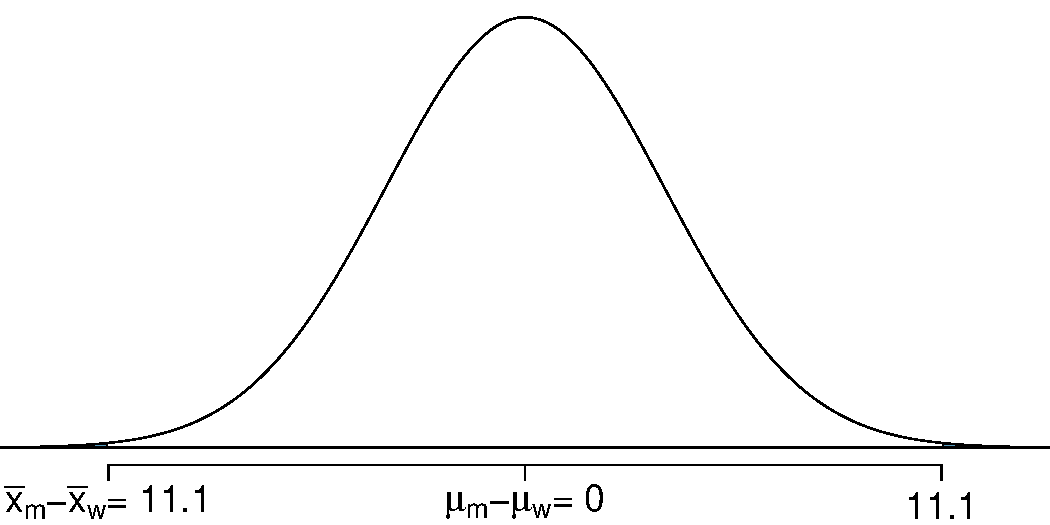
\includegraphics[width=0.75\textwidth]{4-5_inf_other_est/bf.pdf}
\end{center}


\end{enumerate}

\end{frame}

%%%%%%%%%%%%%%%%%%%%%%%%%%%%%%%%%%%

\begin{frame}
\frametitle{Teste de hipóteses para estimativas pontuais quase normais}
\begin{enumerate}
\justifying
\item[5.] A estatística de teste é calculada como a diferença entre a estimativa pontual e o valor nulo (-11.1 - 0 = -11.1), escalada pelo erro padrão.

\[ Z = \frac{11.1 - 0}{0.114} = 97.36 \]
\justifying
O valor de Z é enorme! E, portanto, o p-valor será pequeno, permitindo-nos rejeitar $H_0$ em favor de $H_A$.

\pause

$\:$ \\
\justifying
Esses dados fornecem evidências convincentes de que a média de BF\% de homens e mulheres é diferente.

\end{enumerate}

\end{frame}

%%%%%%%%%%%%%%%%%%%%%%%%%%%%%%%%%%%

\subsection{Estimativas pontuais não normais}

%%%%%%%%%%%%%%%%%%%%%%%%%%%%%%%%%%%

\begin{frame}
\frametitle{Estimativas pontuais não normais}

\begin{itemize}
\justifying
\item Podemos aplicar as ideias de intervalos de confiança e testes de hipóteses aos casos em que a estimativa pontual ou a estatística de teste não é necessariamente normal. Existem muitas razões pelas quais tal situação pode surgir:
\begin{itemize}
\justifying
\item o tamanho da amostra é muito pequeno para que a aproximação normal seja válida;
\justifying
\item a estimativa de erro padrão pode ser ruim; ou
\justifying
\item a estimativa pontual tende para alguma distribuição que não é a distribuição normal.
\end{itemize}
\justifying
\item Para cada caso em que a aproximação normal não é válida, nossa primeira tarefa é sempre entender e caracterizar a distribuição amostral da estimativa pontual ou estatística de teste. Em seguida, podemos aplicar as estruturas gerais para intervalos de confiança e testes de hipóteses a essas distribuições alternativas.

\end{itemize}

\end{frame}

%%%%%%%%%%%%%%%%%%%%%%%%%%%%%%%%%%%

\subsection{Quando recuar}

%%%%%%%%%%%%%%%%%%%%%%%%%%%%%%%%%%%

\begin{frame}
\frametitle{Quando recuar}

\begin{itemize}
\justifying
\item As ferramentas estatísticas dependem das duas condições principais a seguir:
\begin{itemize}
\justifying
\item \hlGr{Independência} Uma amostra aleatória de menos de 10\% da população assegura a independência das observações. Em experimentos, isso é garantido por amostragem aleatória. Se a independência falhar, técnicas avançadas devem ser usadas e, em alguns casos, a inferência pode não ser possível.
\justifying
\item \hlGr{Tamanho e viés da amostra} Por exemplo, se o tamanho da amostra for muito pequeno, o viés muito forte ou valores extremos estiverem presentes, o modelo normal da média da amostra falhará.
\end{itemize}
\end{itemize}

\end{frame}
%%%%%%%%%%%%%%%%%%%%%%%%%%%%%%%%%%%

\begin{frame}
\frametitle{Quando recuar}

\begin{itemize}
\justifying
\item Sempre que as condições não forem satisfeitas para uma técnica estatística:
\begin{enumerate}
\justifying
\item Aprenda novos métodos apropriados para os dados. 
\justifying
\item Consulte um estatístico.
\justifying
\item \sout{Ignorar o fracasso das condições.} Esta última opção efetivamente invalida qualquer análise e pode desacreditar descobertas novas e interessantes.
\end{enumerate}

\end{itemize}

\end{frame}

%%%%%%%%%%%%%%%%%%%%%%%%%%%%%%%%%%%

\subsection{Significância estatística versus significado prático}

%%%%%%%%%%%%%%%%%%%%%%%%%%%%%%%%%%%

\begin{frame}
\frametitle{Prática}
\justifying
\pq{Todo o resto é igual, o p-valor será menor se $n = 100$ ou $n = 10,000$?}

\begin{enumerate}[(a)]
\item $n = 100$
\solnMult{$n = 10,000$}
\end{enumerate}

\soln{\pause \pause
Suponha $\bar{x} = 50$, $s = 2$, $H_0: \mu = 49.5$, e $H_A: \mu > 49.5$.\\
\pause
\begin{eqnarray*}
Z_{n = 100} &=& \frac{50 - 49.5}{\frac{2}{\sqrt{100}}} \pause = \frac{50 - 49.5}{\frac{2}{10}} = \frac{0.5}{0.2} = 2.5,~~~\text{p-valor} = 0.0062 \\
\pause
Z_{n = 10000} &=& \frac{50 - 49.5}{\frac{2}{\sqrt{10000}}} \pause = \frac{50 - 49.5}{\frac{2}{100}} = \frac{0.5}{0.02} = 25,~~~\text{p-valor} \approx 0
\end{eqnarray*}
\pause
\begin{center}
Como $ n $ aumenta - $SE$ $\downarrow$, $Z$ $\uparrow$, p-valor $\downarrow$
\end{center}
}

\end{frame}

%%%%%%%%%%%%%%%%%%%%%%%%%%%%%%%%%%%%

\begin{frame}
\frametitle{Prática}
\justifying
\dq{Teste a hipótese $H_0: \mu = 10$ vs. $H_A: \mu > 10$ para as 8 amostras seguintes. Assuma $\sigma = 2$.}

\begin{center}
\renewcommand\arraystretch{1.5}
\begin{tabular}{l | c | c | c | c}
\hline
$\bar{x}$		& $10.05$ 	& $10.1$ 		& $10.2$  		 \\ 
\hline
\hline
\orange{$n = 30$}  
	& \soln{\only<1>{\textcolor{white}{$p-valor = 0.45$}}		\only<2->{$p-valor = 0.45$}}	
	& \soln{\only<1-3>{\textcolor{white}{$p-valor = 0.39$}}		\only<4->{$p-valor = 0.39$}} 		
	& \soln{\only<1-5>{\textcolor{white}{$p-valor = 0.29$}}		\only<6->{$p-valor = 0.29$}} \\
\hline
\hline
\orange{$n = 5000$} 
	& \soln{\only<1-2>{\textcolor{white}{$p-valor = 0.39$}}		\only<3->{$p-valor = 0.04$}}	
	& \soln{\only<1-4>{\textcolor{white}{$p-valor = 0.0002$}}		\only<5->{$p-valor = 0.0002$}}	
	& \soln{\only<1-6>{\textcolor{white}{$p-valor \approx 0$}}	\only<7->{$p-valor \approx 0$}}	 \\
\hline
\end{tabular}
\end{center}

\pause
\justifying
\soln{\only<8->{Quando $n$ é grande, mesmo pequenos desvios da hipótese nula (tamanhos de efeito pequenos), que podem ser considerados praticamente insignificantes, podem produzir resultados estatisticamente significativos.}}

\end{frame}

%%%%%%%%%%%%%%%%%%%%%%%%%%%%%%%%%%%%

\begin{frame}
\frametitle{Significado estatístico vs. prático}

\begin{itemize}
\justifying
\item Diferenças reais entre a estimativa pontual e a hipótese nula são mais fáceis de detectar com amostras maiores.
\justifying
\item No entanto, amostras muito grandes resultarão em significância estatística mesmo para pequenas diferenças entre a média da amostra e a hipótese nula (\hl{efeito de tamanho}), mesmo quando a diferença não for praticamente significativa.
\justifying
\item Isso é especialmente importante para a pesquisa: se conduzirmos um estudo, queremos nos concentrar em encontrar resultados significativos (queremos que as diferenças observadas sejam reais, mas também grandes o bastante para serem importantes).
\justifying
\item O papel de um estatístico não é apenas na análise de dados, mas também no planejamento e projeto de um estudo.
\end{itemize}

\end{frame}
%%%%%%%%%%%%%%%%%%%%%%%%%%%%%%%%%%%%
\begin{frame}
\frametitle{Significado estatístico vs. prático}

\justifying
\begin{center}{\footnotesize
\textit{``Chamar o estatístico após o término do experimento pode não ser mais do que pedir que ele faça um exame post-mortem: ele pode ser capaz de lhe dizer porque o experimento morreu.''} -- R.A. Fisher
}\end{center}

\end{frame}

%%%%%%%%%%%%%%%%%%%%%%%%%%%%%%%%%%%%

